\documentclass[12pt, a4paper, twoside]{report}
\usepackage[utf8]{inputenc}
\usepackage[T1,T2A]{fontenc}

\usepackage[russian, english]{babel}
\usepackage{xcolor} %for transparency
\usepackage{graphicx}

\usepackage{indentfirst}

\newcommand{\HRule}{\rule{\linewidth}{0.5mm}}
%\setcounter{section}{1}
\renewcommand{\thesection}{\arabic{section}}

%Rename contents - magic here
\addto\captionsenglish{% Replace "english" with the language you use
	  \renewcommand{\contentsname}%
	      {Оглавление}%
      }
%END rename contents

\begin{document}

\begin{titlepage}
\begin{center}
\fontencoding{T1}\selectfont

\textsc{\LARGE Liceum Boarding School number 2}\\[1.5cm]

\textsc{\Large Some crappy project}\\[0.5cm]

% Title
\HRule \\[0.4cm]
{ \huge \bfseries Tesseract and hyperplane investigation\\[0.4cm] }

\HRule \\[1.5cm]

% Author and supervisor
\noindent
\begin{minipage}{0.4\textwidth}
\begin{flushleft} \large
\emph{Authors:}\\
Ilgic \textsc{Mustafin} \newline
\fontencoding{T2A}\selectfont
Гриша \textsc{Maxxx} \newline %USE RUSSIAN FONT
\fontencoding{T1}\selectfont %USE LATIN HERE
Mirolin \textsc{M} 
and \newline
Arthur \textsc{Nugmanov} 
\end{flushleft}
\end{minipage}%
\begin{minipage}{0.4\textwidth}
\begin{flushright} \large
\emph{Supervisor:} \\
Marsel \textsc{Abiy}
\end{flushright}
\end{minipage}

\vfill

% Bottom of the page
{\large \today}

\end{center}
\end{titlepage}
 %Load titlepage so we do not mess up the numeration

\tableofcontents

\newpage
\section{Введение}
Введение, тезисы, примерное описание работы.
Данная работа ставит своей целью создать математическую модель пересечения четырехмерного гиперкуба или тессеракта трехмерной гиперплоскость, а также создать программную имплементацию данной математической задачи. Предполагается рассмотреть варианты возможных сечений данного гиперкуба.

Как известно, гиперкуб представляет собой куб в четырехмером пространстве, может также называться тетракубом и тессерактом. В даннной работе будет рассматриваться представление данной фигуры в виде множества точек $(x_1,x_2,x_3,x_4)\in R^4$ таких что $\|x_i\|\leq 1$. Тессеракт ограничивают 8 гиперплоскостей, т.е.подпространств, на единицу меньшей чем объемлющее пространство.

\begin{figure}[h!]
	\center
	\framebox{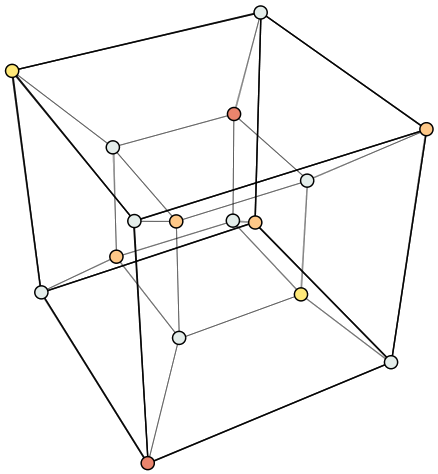
\includegraphics[scale=0.5]{./tesseract_fig1.png}}
	\clearpage
\end{figure}
\section{Тессеракт, или четырехмерный гиперкуб}
Конечно, невозможно представить графически, как будет выглядеть данный гиперкуб в четырехмерном пространстве, не выходя из трехмерного. Можно лишь представить проекцию данного тессеракта на трехмерныю плоскость. В случае проекции невозможно определить точки сечения, поэтому все действия нами выполнялись в четырехмерных координатах для получения трехмерного сечения, представляющего из себя многогранник.

Далее будет рассмотрен довольно простой способ представления проекции тессеракта на трехмерную плоскость. Этот метод позволяет представить примерно, как выглядит рабочий куб, но, как уже отмечалось выше, данный метод не позволяет определить точки пересечения гиперплоскости с четырехмерным кубом.
\subsection{Построение проекции гиперкуба на плоскость}
Попытаемся представить себе, как будет выглядеть гиперкуб, не выходя из трёхмерного пространства. Возьмем одномерное пространство (линию), выделим на нем отрезок длиной $а$. Теперь перенесем его на двумерную плоскость и на расстоянии $а$ от него нарисуем параллельный ему отрезок той же длины, затем соединим концы. Получится квадрат. Повторив эту операцию с двумерной плоскостью, получим трехмерный куб, а если применить ту же операцию к трехмерному пространству, то получится гиперкуб т.е. его можно представить, как два трехменых куба, лежащих в парралельных трехмерных пространствах, с попарно соединенными вершинами. 

\begin{figure}[h!]
	\framebox{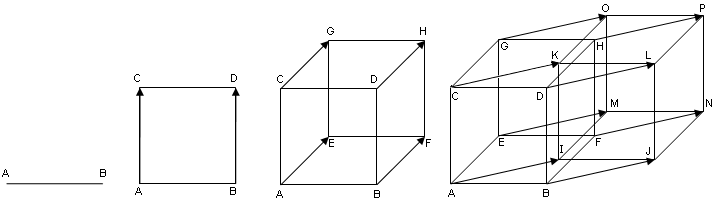
\includegraphics[scale=0.6]{./make_tess.png}}
	\clearpage
\end{figure}

Если задуматься о том, как будет выглядеть сечение тессеракта в четырехмерном пространстве, можно прийти к следующей аналогии: сечением одномерного объекта будет точка, двумерного -  отрезок, трехмерного - плоскость. По аналогии сечением четырехмерного объекта является трехмерный объект. Наша задача состоит как раз в отыскании принципа построения данных сечений.

\section{Мат. аппарат}
Перейдем к описанию математической модели построения данных сечений.
\section{Описание работы программы}
\section{Примеры сечений}
\subsection{Тетраэдр}

\subsection{Пятигранная призма}
\subsection{Шестигранная призма}
0 1 0 1
1 0 1 1
0 1 1 1
0 0 0 0
\section{Тессеракт в культуре}
\subsection{В литература}
\subsection{В кинематографе}
\subsection{В мифологии(прим. жидорептилоиды)}
\section{Заключение}
\section{Список используемой литературы}
\section{Приложения}

\end{document}

